% Options for packages loaded elsewhere
\PassOptionsToPackage{unicode}{hyperref}
\PassOptionsToPackage{hyphens}{url}
\PassOptionsToPackage{dvipsnames,svgnames,x11names}{xcolor}
%
\documentclass[
  notoc,
  nobib,
  degree=inf]{mnye}
\usepackage{amsmath,amssymb}
\usepackage{lmodern}
\usepackage{iftex}
\ifPDFTeX
  \usepackage[T1]{fontenc}
  \usepackage[utf8]{inputenc}
  \usepackage{textcomp} % provide euro and other symbols
\else % if luatex or xetex
  \usepackage{unicode-math}
  \defaultfontfeatures{Scale=MatchLowercase}
  \defaultfontfeatures[\rmfamily]{Ligatures=TeX,Scale=1}
\fi
% Use upquote if available, for straight quotes in verbatim environments
\IfFileExists{upquote.sty}{\usepackage{upquote}}{}
\IfFileExists{microtype.sty}{% use microtype if available
  \usepackage[]{microtype}
  \UseMicrotypeSet[protrusion]{basicmath} % disable protrusion for tt fonts
}{}
\makeatletter
\@ifundefined{KOMAClassName}{% if non-KOMA class
  \IfFileExists{parskip.sty}{%
    \usepackage{parskip}
  }{% else
    \setlength{\parindent}{0pt}
    \setlength{\parskip}{6pt plus 2pt minus 1pt}}
}{% if KOMA class
  \KOMAoptions{parskip=half}}
\makeatother
\usepackage{xcolor}
\IfFileExists{xurl.sty}{\usepackage{xurl}}{} % add URL line breaks if available
\IfFileExists{bookmark.sty}{\usepackage{bookmark}}{\usepackage{hyperref}}
\hypersetup{
  pdftitle={Inferencia estadística},
  pdfauthor={Eva María Mazcuñán Navarro},
  colorlinks=true,
  linkcolor={Maroon},
  filecolor={Maroon},
  citecolor={Blue},
  urlcolor={Blue},
  pdfcreator={LaTeX via pandoc}}
\urlstyle{same} % disable monospaced font for URLs
\usepackage{color}
\usepackage{fancyvrb}
\newcommand{\VerbBar}{|}
\newcommand{\VERB}{\Verb[commandchars=\\\{\}]}
\DefineVerbatimEnvironment{Highlighting}{Verbatim}{commandchars=\\\{\}}
% Add ',fontsize=\small' for more characters per line
\usepackage{framed}
\definecolor{shadecolor}{RGB}{248,248,248}
\newenvironment{Shaded}{\begin{snugshade}}{\end{snugshade}}
\newcommand{\AlertTok}[1]{\textcolor[rgb]{0.94,0.16,0.16}{#1}}
\newcommand{\AnnotationTok}[1]{\textcolor[rgb]{0.56,0.35,0.01}{\textbf{\textit{#1}}}}
\newcommand{\AttributeTok}[1]{\textcolor[rgb]{0.77,0.63,0.00}{#1}}
\newcommand{\BaseNTok}[1]{\textcolor[rgb]{0.00,0.00,0.81}{#1}}
\newcommand{\BuiltInTok}[1]{#1}
\newcommand{\CharTok}[1]{\textcolor[rgb]{0.31,0.60,0.02}{#1}}
\newcommand{\CommentTok}[1]{\textcolor[rgb]{0.56,0.35,0.01}{\textit{#1}}}
\newcommand{\CommentVarTok}[1]{\textcolor[rgb]{0.56,0.35,0.01}{\textbf{\textit{#1}}}}
\newcommand{\ConstantTok}[1]{\textcolor[rgb]{0.00,0.00,0.00}{#1}}
\newcommand{\ControlFlowTok}[1]{\textcolor[rgb]{0.13,0.29,0.53}{\textbf{#1}}}
\newcommand{\DataTypeTok}[1]{\textcolor[rgb]{0.13,0.29,0.53}{#1}}
\newcommand{\DecValTok}[1]{\textcolor[rgb]{0.00,0.00,0.81}{#1}}
\newcommand{\DocumentationTok}[1]{\textcolor[rgb]{0.56,0.35,0.01}{\textbf{\textit{#1}}}}
\newcommand{\ErrorTok}[1]{\textcolor[rgb]{0.64,0.00,0.00}{\textbf{#1}}}
\newcommand{\ExtensionTok}[1]{#1}
\newcommand{\FloatTok}[1]{\textcolor[rgb]{0.00,0.00,0.81}{#1}}
\newcommand{\FunctionTok}[1]{\textcolor[rgb]{0.00,0.00,0.00}{#1}}
\newcommand{\ImportTok}[1]{#1}
\newcommand{\InformationTok}[1]{\textcolor[rgb]{0.56,0.35,0.01}{\textbf{\textit{#1}}}}
\newcommand{\KeywordTok}[1]{\textcolor[rgb]{0.13,0.29,0.53}{\textbf{#1}}}
\newcommand{\NormalTok}[1]{#1}
\newcommand{\OperatorTok}[1]{\textcolor[rgb]{0.81,0.36,0.00}{\textbf{#1}}}
\newcommand{\OtherTok}[1]{\textcolor[rgb]{0.56,0.35,0.01}{#1}}
\newcommand{\PreprocessorTok}[1]{\textcolor[rgb]{0.56,0.35,0.01}{\textit{#1}}}
\newcommand{\RegionMarkerTok}[1]{#1}
\newcommand{\SpecialCharTok}[1]{\textcolor[rgb]{0.00,0.00,0.00}{#1}}
\newcommand{\SpecialStringTok}[1]{\textcolor[rgb]{0.31,0.60,0.02}{#1}}
\newcommand{\StringTok}[1]{\textcolor[rgb]{0.31,0.60,0.02}{#1}}
\newcommand{\VariableTok}[1]{\textcolor[rgb]{0.00,0.00,0.00}{#1}}
\newcommand{\VerbatimStringTok}[1]{\textcolor[rgb]{0.31,0.60,0.02}{#1}}
\newcommand{\WarningTok}[1]{\textcolor[rgb]{0.56,0.35,0.01}{\textbf{\textit{#1}}}}
\usepackage{longtable,booktabs,array}
\usepackage{calc} % for calculating minipage widths
% Correct order of tables after \paragraph or \subparagraph
\usepackage{etoolbox}
\makeatletter
\patchcmd\longtable{\par}{\if@noskipsec\mbox{}\fi\par}{}{}
\makeatother
% Allow footnotes in longtable head/foot
\IfFileExists{footnotehyper.sty}{\usepackage{footnotehyper}}{\usepackage{footnote}}
\makesavenoteenv{longtable}
\usepackage{graphicx}
\makeatletter
\def\maxwidth{\ifdim\Gin@nat@width>\linewidth\linewidth\else\Gin@nat@width\fi}
\def\maxheight{\ifdim\Gin@nat@height>\textheight\textheight\else\Gin@nat@height\fi}
\makeatother
% Scale images if necessary, so that they will not overflow the page
% margins by default, and it is still possible to overwrite the defaults
% using explicit options in \includegraphics[width, height, ...]{}
\setkeys{Gin}{width=\maxwidth,height=\maxheight,keepaspectratio}
% Set default figure placement to htbp
\makeatletter
\def\fps@figure{htbp}
\makeatother
\setlength{\emergencystretch}{3em} % prevent overfull lines
\providecommand{\tightlist}{%
  \setlength{\itemsep}{0pt}\setlength{\parskip}{0pt}}
\setcounter{secnumdepth}{5}
\usepackage{ehyperref}
\colorlet{etoccolor}{greenlink}
% This file is created the first time epdf_document is invoked
% but will not be overwriten afterwards.
%
% Preamble

\usepackage{ebox}
\usepackage{enotation}
\usepackage{fontawesome}

% https://stackoverflow.com/questions/63222203/rmarkdown-wrap-code-in-chunks-but-keep-breaks-after-pipe
\usepackage{fvextra}
\DefineVerbatimEnvironment{Highlighting}{Verbatim}{
    breaksymbolleft={},
    showspaces = false,
    showtabs = false,
    breaklines,
    commandchars=\\\{\}
}

\pgfplotsset{compat=1.18}


\renewcommand\cfttocprehook{
%     \cleardoublepage%
    \pagenumbering{roman}%
    \pagestyle{plain}%
}

\renewcommand\cfttocposthook{
    \cleardoublepage%
    \pagenumbering{arabic}%
    \pagestyle{main}%
}

% highr::hi_latex(..., markup = cmd_pandoc_latex)
% `...`{.R}
\renewcommand{\DecValTok}[1]{\textcolor[RGB]{64, 160, 112}{\texttt{#1}}}
\renewcommand{\FloatTok}[1]{\textcolor[RGB]{64, 160, 112}{\texttt{#1}}}
\renewcommand{\FunctionTok}[1]{\textcolor[rgb]{0.13,0.29,0.53}{\texttt{#1}}}
\renewcommand{\KeywordTok}[1]{\textcolor[rgb]{0.13,0.29,0.53}{\texttt{#1}}}
\renewcommand{\NormalTok}[1]{\texttt{#1}}
\pretitle{TEMA 8}
\degree{inf}
\term{2021-2022}
\ifLuaTeX
  \usepackage{selnolig}  % disable illegal ligatures
\fi
\usepackage[]{biblatex}
\addbibresource{bib/book.bib}
\addbibresource{bib/packages.bib}
\addbibresource{bib/Estadistica.bib}

\title{Inferencia estadística}
\author{Eva María Mazcuñán Navarro}
\date{}

\begin{document}
\maketitle

% This file is created the first time epdf_document is invoked
% but will not be overwriten afterwards.
%
% Before Body

{
\hypersetup{linkcolor=etoccolor}
\setcounter{tocdepth}{2}
\tableofcontents
}
\hypertarget{section}{%
\section*{}\label{section}}

\hypertarget{intro}{%
\section*{Introducción}\label{intro}}
\addcontentsline{toc}{section}{Introducción}



\begin{figure}

{\centering 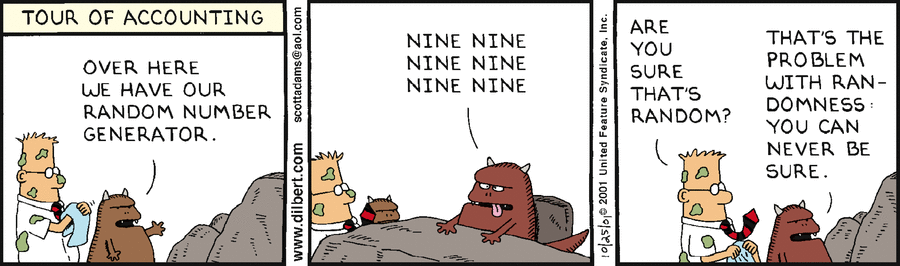
\includegraphics[width=1\linewidth]{graficos/dilbertc} 

}

\caption{Viñeta de la tira cómica \emph{Dilbert}, de Scott Adams.}\label{fig:dilbert}
\end{figure}



\begin{figure}

{\centering 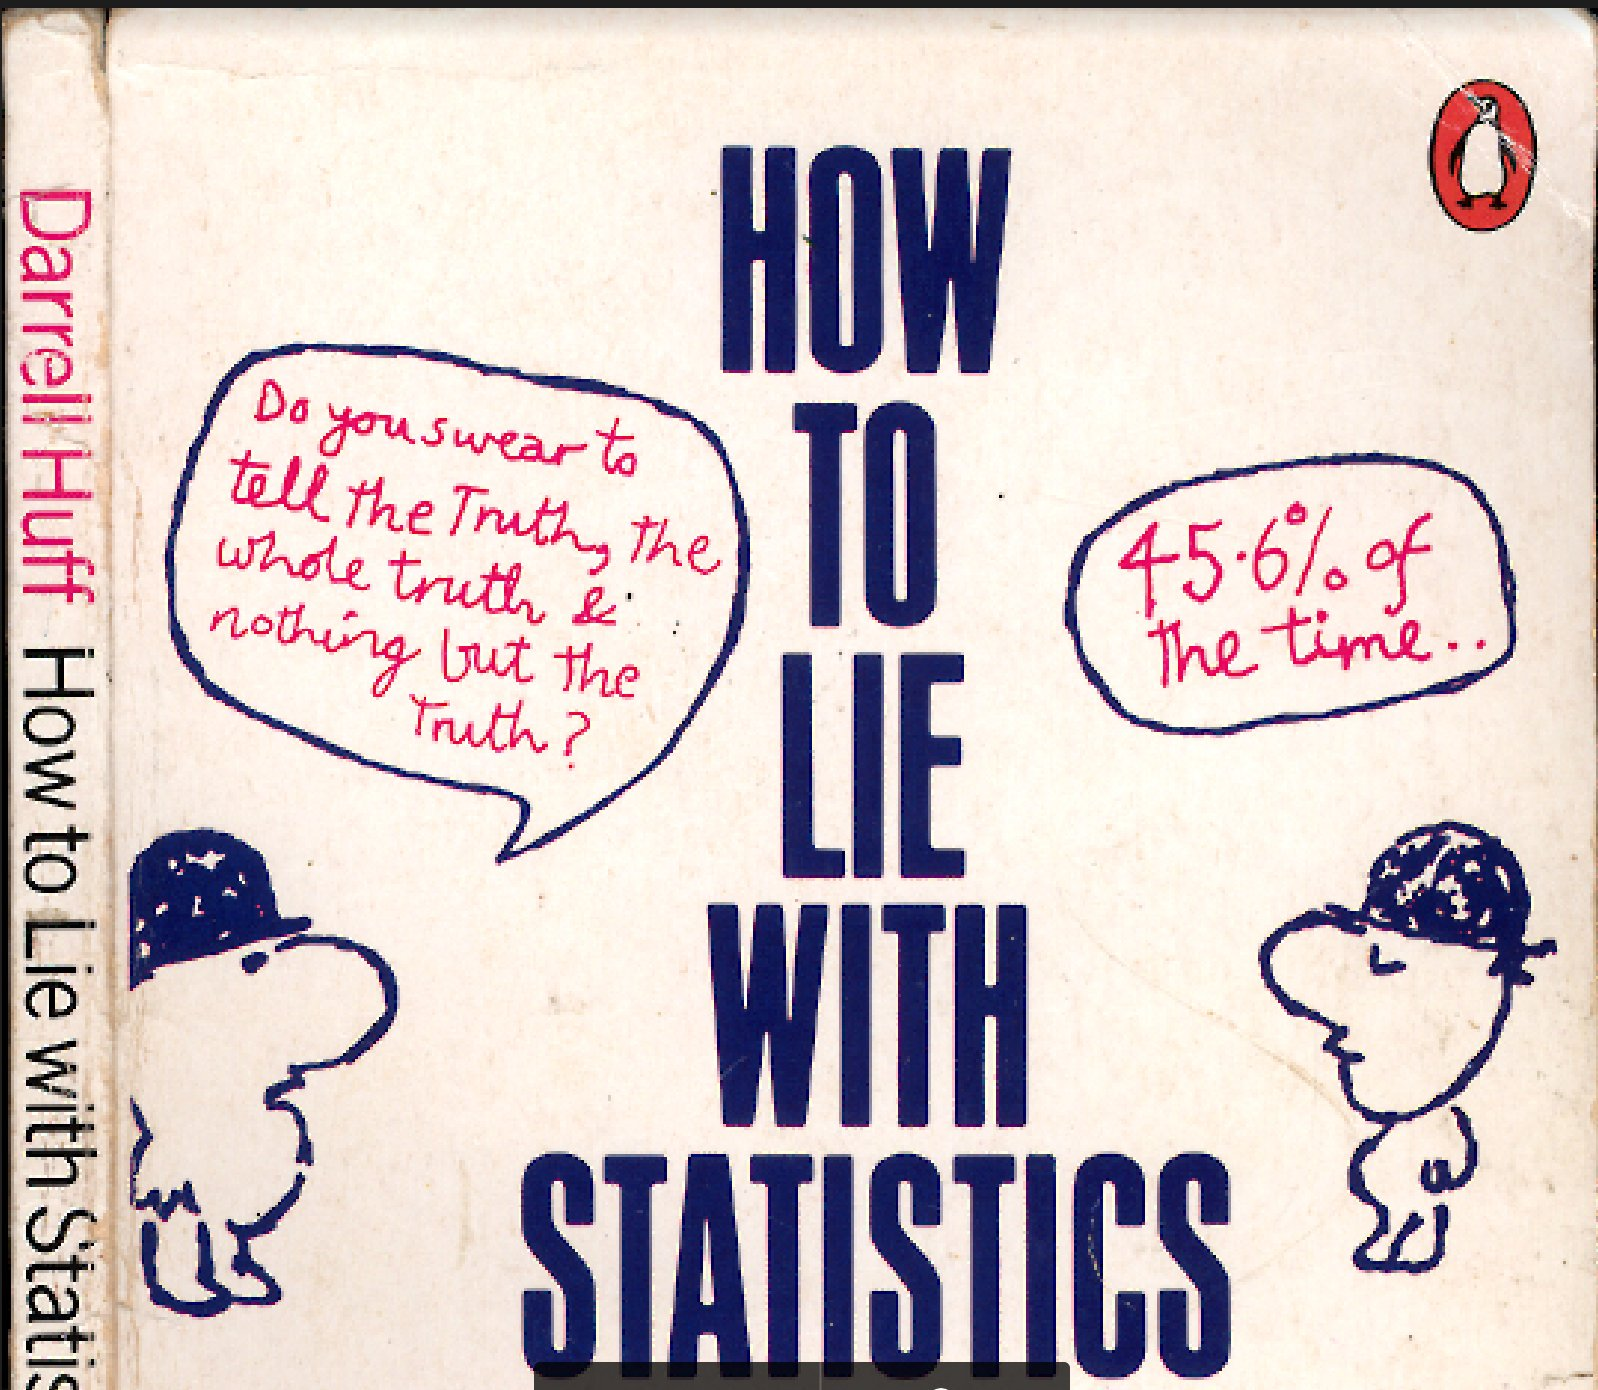
\includegraphics[width=0.7\linewidth]{graficos/HowToLieWithStatistics4} 

}

\caption{Portada del libro \emph{How to Lie with Statistics}, de Darrell Huff.}\label{fig:lie}
\end{figure}

Hasta ahora hemos realizado un estudio teórico de las variables aleatorias. Y hemos aprendido a resolver problemas como el siguiente:

\begin{ebox}{}
Sabemos que, para un determinado jugador de baloncesto, la probabilidad con que acierta un lanzamiento de tiro libre es \(0.75\).

Calcula la probabilidad de que, en una tanda de \(50\) lanzamientos, acierte como máximo \(30\) de ellos.

\end{ebox}

Para resolver el problema anterior, consideramos la variable aleatoria

\begin{center}
\(X =\) número de lanzamientos acertados.

\end{center}

Identificamos que \(X\) sigue una distribución binomial de parámetros \(n=50\) y \(p=0.75\), abreviadamente \[X\sim Binom(50,0.75),\] y calculamos la probabilidad pedida como

\[
  P(X\le 30) = F(30) =  \KeywordTok{pbinom}\NormalTok{(}\DecValTok{30}\NormalTok{,} \DecValTok{50}\NormalTok{,} \DecValTok{0.75}\NormalTok{)} = 0.0139.
\]

Ahora, en una situación real, lo más frecuente es que no conozcamos el valor \(p=0.75\) para la probabilidad de acierto del jugador en el lanzamiento de tiros libres. Porque este valor \(p\) es un parámetro teórico, que interpretamos como la proporción de aciertos del jugador cuando el número de lanzamientos tiende a infinito. Para obtener el valor de \(p\) deberíamos observar los infinitos potenciales lanzamientos que podría efectuar el lanzador, situación imposible en la práctica. En consecuencia, el tipo de problema que se plantea en la práctica es más parecido al siguiente:

\begin{ex}

Nos planteamos investigar el valor del parámetro

\begin{center}{}
{\(p =\)} probabilidad de que el jugador acierte un tiro libre.

\end{center}

Para ello, observamos el resultado de \(50\) lanzamientos efectuados por el jugador en cuestión, anotando en cada caso si acierta o falla. Se obtienen \(28\) aciertos y \(22\) fallos.

El objetivo es realizar inferencias sobre el parámetro \(p\) basándonos en los resultados de los lanzamientos observados. Queremos en concreto responder a las siguientes cuestiones:

\begin{itemize}
\item
  El jugador afirma que su probabilidad de acertar un tiro libre es \(0.75\) ¿resultan los datos compatibles con esta afirmación?
\item
  A la vista de los datos ¿cuál sería un rango de valores plausibles para la probabilidad \(p\)?
\end{itemize}

\end{ex}

En este tema estudiaremos los procedimientos de inferencia estadística que permitirán responder a las preguntas anteriores. Responderemos a la primera pregunta utilizando un procedimiento de inferencia estadística denominado \textbf{contraste de hipótesis} (sección \ref{hypothesis}) y abordaremos la segunda cuestión construyendo un \textbf{intervalo de confianza} (sección \ref{conf-int}).

En general, un procedimiento de inferencia estadística es un método o técnica que permite inferir, a partir de la información empírica proporcionada por una muestra (en nuestro ejemplo los aciertos observados en \(50\) lanzamientos), el comportamiento de una determinada población (en nuestro ejemplo la probabilidad de acierto \(p\)). Las conclusiones de un procedimiento de inferencia estadística nunca serán afirmaciones categóricas, sino que estarán sujetas a un riesgo de error, que se cuantifica en términos de probabilidades (ver figuras \ref{fig:dilbert} y \ref{fig:lie}).

Presentaremos el comando de \textsf{R} \VERB|\FunctionTok{binom.test}\NormalTok{()}| para realizar el contraste de hipótesis y obtener el intervalo de confianza para la proporción \(p\) que responderán a las preguntas planteadas antes. Basándonos en nuestro conocimiento de las variables binomiales estudiadas en el tema anterior, seremos capaces de reproducir los cálculos que realiza este comando. De esta forma, podremos entender los fundamentos generales de los contrastes de hipótesis y los intervalos de confianza.

En la última práctica de ordenador del curso, estudiaremos más comandos de \textsf{R} para realizar contrastes de hipótesis y calcular intervalos de confianza para otros parámetros, como la media de una variable continua. Gracias a lo aprendido en este tema, sabremos interpretar las salidas de dichos comandos, aún sin conocer el detalle de los cálculos realizados para obtenerlas.

\hypertarget{descriptive}{%
\section{Estadística descriptiva}\label{descriptive}}

Todo estudio estadístico comienza con una exploración inicial de los datos obtenidos, que habitualmente incluye el cálculo determinados valores de interés que resumen o describen los datos, y la visualización de los datos mediante los gráficos adecuados en cada caso.

Para nuestro ejemplo calcularemos la llamada proporción muestral y realizaremos un diagrama de barras.

Comenzamos cargando el paquete \texttt{tidyverse} para tener acceso a todas las funciones de \textsf{R} que usaremos a lo largo del tema.

\begin{Shaded}
\begin{Highlighting}[]
\FunctionTok{library}\NormalTok{(}\StringTok{"tidyverse"}\NormalTok{)}
\end{Highlighting}
\end{Shaded}

\hypertarget{point}{%
\subsection{Estimación puntual}\label{point}}

Supongamos, como se indicó en el problema planteado en la introducción, que en los \(50\) lanzamientos observados, el jugador acertó \(28\) de ellos (y falló los \(22\) restantes).

Recordemos que nuestro objetivo es estimar el valor teórico de la probabilidad o proporción de aciertos \(p\) del jugador. Una forma natural de hacerlo es calcular la proporción de aciertos en nuestra muestra de \(50\) lanzamientos: \[
 \hat{p} = \frac{28}{50} = 0.56.
\]

Este valor se denomina \textbf{proporción muestral} y se denota \(\widehat{p}\), porque nos da una idea aproximada de cuál puede ser el verdadero valor del valor teórico \(p\), que se llama \textbf{proporción poblacional}.

Decimos que la proporción muestral \(\widehat{p} = 0.56\) es una \textbf{estimación puntual} de la proporción poblacional \(p\). En general, una estimación puntual de un parámetro es un valor numérico calculado a partir de la muestra que nos orienta sobre el verdadero valor del parámetro.

Hay que tener claro que la proporción muestral \(\widehat{p}=0.56\) nos proporciona una estimación puntual de la proporción poblacional \(p\), pero que el verdadero valor de \(p\) sigue siendo desconocido. El verdadero valor de \(p\) es la probabilidad de que el jugador acierte un tiro libre, que identificamos con la proporción de aciertos en el conjunto ideal de los infinitos lanzamientos que podría efectuar el jugador. Por su parte, el valor \(\widehat{p}=0.56\) es tan sólo la proporción de aciertos en los \(50\) lanzamientos que hemos observado. Podría ser que los \(50\) lanzamientos observados sean una ``mala racha'', y que el verdadero valor de la proporción de aciertos \(p\) sea superior a \(\widehat{p}=0.56\).

\hypertarget{gruxe1ficos}{%
\subsection{Gráficos}\label{gruxe1ficos}}

Ahora vamos a representar gráficamente los datos mediante un diagrama de barras.

En primer lugar creamos una tabla con el recuento de aciertos y fallos:

\begin{Shaded}
\begin{Highlighting}[]
\NormalTok{basket }\OtherTok{\textless{}{-}} \FunctionTok{tibble}\NormalTok{(}
  \AttributeTok{result =} \FunctionTok{c}\NormalTok{(}\StringTok{"Acierto"}\NormalTok{, }\StringTok{"Fallo"}\NormalTok{),}
  \AttributeTok{count =} \FunctionTok{c}\NormalTok{(}\DecValTok{28}\NormalTok{, }\DecValTok{22}\NormalTok{)}
\NormalTok{)}
\end{Highlighting}
\end{Shaded}

Y usamos la tabla creada para crear un diagrama de barras con la función \VERB|\FunctionTok{geom\_col}\NormalTok{()}|:

\begin{Shaded}
\begin{Highlighting}[]
\FunctionTok{ggplot}\NormalTok{(}
  \AttributeTok{data =}\NormalTok{ basket,}
  \AttributeTok{mapping =} \FunctionTok{aes}\NormalTok{(}
    \AttributeTok{x =}\NormalTok{ result,}
    \AttributeTok{y =}\NormalTok{ count}
\NormalTok{  )}
\NormalTok{) }\SpecialCharTok{+}
  \FunctionTok{geom\_col}\NormalTok{()}
\end{Highlighting}
\end{Shaded}

\begin{center}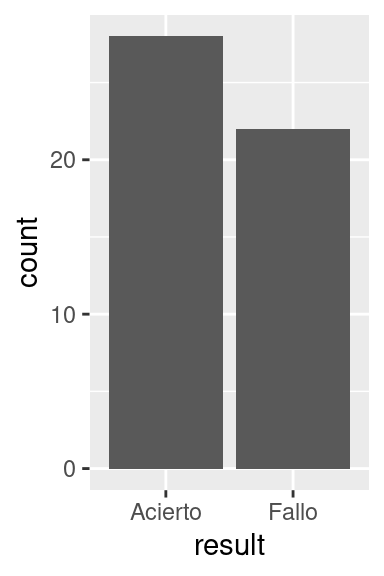
\includegraphics[width=0.31\linewidth]{T8-Inferencia_files/figure-latex/unnamed-chunk-8-1} \end{center}

Mejoramos un poco el aspecto inicial de nuestro gráfico de barras añadiendo rótulos, cambiando el color de las barras, y girándolo con \VERB|\FunctionTok{coord\_flip}\NormalTok{()}|:

\begin{Shaded}
\begin{Highlighting}[]
\FunctionTok{ggplot}\NormalTok{(}
  \AttributeTok{data =}\NormalTok{ basket,}
  \AttributeTok{mapping =} \FunctionTok{aes}\NormalTok{(}
    \AttributeTok{x =}\NormalTok{ result,}
    \AttributeTok{y =}\NormalTok{ count}
\NormalTok{  )}
\NormalTok{) }\SpecialCharTok{+}
  \FunctionTok{geom\_col}\NormalTok{(}
    \AttributeTok{fill =} \StringTok{"\#7AA3E5"}
\NormalTok{  ) }\SpecialCharTok{+}
  \FunctionTok{coord\_flip}\NormalTok{() }\SpecialCharTok{+}
  \FunctionTok{labs}\NormalTok{(}
    \AttributeTok{title =} \StringTok{"Resultado de 50 tiros libres"}\NormalTok{,}
    \AttributeTok{x =} \StringTok{""}\NormalTok{,}
    \AttributeTok{y =} \StringTok{"Recuento"}
\NormalTok{  ) }\SpecialCharTok{+}
  \FunctionTok{theme}\NormalTok{(}\AttributeTok{plot.title =} \FunctionTok{element\_text}\NormalTok{(}\AttributeTok{hjust =} \FloatTok{0.5}\NormalTok{)) }\CommentTok{\# centrar título}
\end{Highlighting}
\end{Shaded}

\begin{center}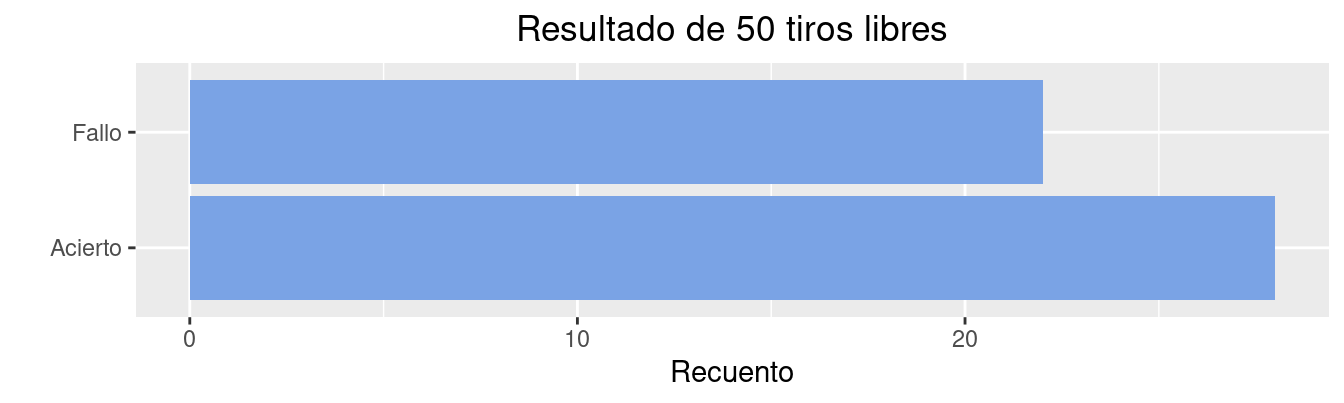
\includegraphics[width=0.8\linewidth]{T8-Inferencia_files/figure-latex/unnamed-chunk-9-1} \end{center}

\hypertarget{hypothesis}{%
\section{Contrastes de hipótesis}\label{hypothesis}}

Hasta ahora hemos descrito los datos numérica y gráficamente. Concretamente, hemos calculado la proporción de aciertos en la muestra, obteniendo el valor \(\widehat{p}=0.56\) para la proporción muestral, como estimación de la proporción poblacional \(p\), y hemos realizado un diagrama de barras de los recuentos de aciertos y fallos.

Nos planteamos ahora responder a la primera cuestión planteada en el problema de la introducción:

\begin{ebox}{}
Supongamos que el jugador afirma que su probabilidad de acertar un tiro libre es \(0.75\). El objetivo es contrastrar si los datos observados resultan compatibles con la afirmación del jugador.

\end{ebox}

Con la exploración inicial que hemos hecho de los datos, podemos concretar el objetivo planteando lo que en estadística se denomina un \textbf{contraste de hipótesis}. Dividiremos el procedimiento en tres pasos: planteamiento de las hipótesis, cálculo del \(p\)-valor y conclusión.

\hypertarget{planteamiento-de-las-hipuxf3tesis}{%
\subsection{Planteamiento de las hipótesis}\label{planteamiento-de-las-hipuxf3tesis}}

Según el jugador la proporción verdadera es \(p=0.75\). Y la estimación de \(p\) según nuestra muestra es \(\widehat{p}=0.56\), inferior al valor de \(p\) según el jugador.

Como resaltamos antes, no podemos concluir con seguridad, basándonos en los datos obtenidos en la muestra de \(50\) lanzamientos, que el jugador mienta. Puede que el jugador diga la verdad, y que, por azar, hayamos observado una racha peor de lo habitual.

Pero nuestros datos levantan la sospecha de que el jugador exagera, y nos sugieren que \(p<0.75\). Esta hipótesis sugerida por los datos se denomina \textbf{hipótesis alternativa}, y se denota \(H_1\).

Por otra parte, a la igualdad \(p=0.75\), se le llama \textbf{hipótesis nula} y se denota \(H_0\).

Resumimos el contraste de hipótesis que planteamos escribiendo

\[
  \left\{
  \begin{array}{lrcl}
    H_0:&p&=&0.75\\
    H_1:&p&<&0.75.
  \end{array}
  \right.
\]

\hypertarget{cuxe1lculo-del-p-valor}{%
\subsection{\texorpdfstring{Cálculo del \(p\)-valor}{Cálculo del p-valor}}\label{cuxe1lculo-del-p-valor}}

Vamos a resolver el conflicto, entre la hipótesis nula \(H_0\), y la hipótesis alternativa \(H_1\) que sugieren los datos, contestando a la pregunta siguiente:

\begin{ebox}{}
Si la realidad fuera que \(p=0.75\) (la hipótesis nula es cierta, el jugador dice la verdad) ¿cuál es la probabilidad de observar una racha tan mala como la observada o peor?

\end{ebox}

Respondiendo a esta pregunta, cuantificaremos la sospecha que han levantado nuestros datos y que provocó la formulación de la hipótesis alternativa.

Si la respuesta es que la probabilidad es muy baja, tomaremos la decisión de acusar de mentiroso al jugador y nos decantaremos por la hipótesis alternativa de que \(p<0.75\). Si por el contrario la probabilidad no es muy baja, lo dejaremos estar y no acusaremos al jugador de mentiroso, pensaremos que los datos observados pueden deberse al azar y no a que el jugador mienta.

Adoptaremos una actitud conservadora, y fijaremos el umbral de lo que consideramos una probabilidad muy baja en \(0.05\). De esta manera, si los datos observados tienen una probabilidad superior a \(0.05\), no acusaremos de mentiroso al jugador. Esta probabilidad se llama \textbf{nivel de significación} del contraste y se denota \(\alpha\). Lo más frecuente en el ámbito científico es trabajar con este nivel de significación \(\alpha=0.05\), pero también pueden convenirse otros valores como \(\alpha=0.01\).

El procedimiento estadístico con el que vamos a resolver el contraste de hipótesis que hemos planteado y a calcular la probabilidad que buscamos se llama \textbf{test binomial exacto}. El comando de \textsf{R} que lo lleva a cabo es \VERB|\FunctionTok{binom.test}\NormalTok{()}|. Concretamente para resolver nuestro contraste tenemos que ejecutar:

\begin{Shaded}
\begin{Highlighting}[]
\FunctionTok{binom.test}\NormalTok{(}
  \AttributeTok{x =} \DecValTok{28}\NormalTok{,}
  \AttributeTok{n =} \DecValTok{50}\NormalTok{,}
  \AttributeTok{p =} \FloatTok{0.75}\NormalTok{,}
  \AttributeTok{alternative =} \StringTok{"less"}
\NormalTok{)}
\end{Highlighting}
\end{Shaded}

\begin{Shaded}
\begin{Highlighting}[]
\NormalTok{\#\# }
\NormalTok{\#\#  Exact binomial test}
\NormalTok{\#\# }
\NormalTok{\#\# data:  28 and 50}
\NormalTok{\#\# number of successes = 28, number of trials = 50, p{-}value = 0.002618}
\NormalTok{\#\# alternative hypothesis: true probability of success is less than 0.75}
\NormalTok{\#\# 95 percent confidence interval:}
\NormalTok{\#\#  0.0000000 0.6801741}
\NormalTok{\#\# sample estimates:}
\NormalTok{\#\# probability of success }
\NormalTok{\#\#                   0.56}
\end{Highlighting}
\end{Shaded}

Los argumentos \texttt{x\ =\ 28} y \texttt{n\ =\ 50} indican que hemos observado \(28\) aciertos en \(50\) lanzamientos. Con el argumento \texttt{p\ =\ 0.75} indicamos que queremos comparar nuestros datos con el valor de referencia \(0.75\) de la hipótesis nula. Y el argumento \texttt{alternative\ =\ "less"} indica que nuestra hipótesis alternativa es que \(p\) es menor que el valor umbral \(0.75\).

La probabilidad que buscamos la encontramos en el fragmento de la salida

\begin{center}
\texttt{p-value = 0.002618.}

\end{center}

Esta probabilidad 0.002618 asociada a nuestro contraste de hipótesis se denomina \textbf{\(\mathbf{p}\)-valor}. La letra \(p\) en \(p\)-valor es inicial de probabilidad, no tiene que ver con que estemos realizando un contraste de hipótesis sobre el parámetro \(p\) (en un contraste de hipótesis para una media también hablaríamos del \(p\)-valor de ese contraste).

En el apartado siguiente, utilizaremos el \(p\)-valor para decidir entre las hipótesis contrastadas, esto es, entre la hipótesis nula \(p=0.75\) y la hipótesis alternativa sugerida por los datos \(p<0.75\). Para entender el criterio que seguiremos, vamos a analizar cómo se calcula el \(p\)-valor que hemos obtenido con \VERB|\FunctionTok{binom.test}\NormalTok{()}|.

El \(p\)-valor \(0.002618\) que hemos obtenido con la función \VERB|\FunctionTok{binom.test}\NormalTok{()}| cuantifica nuestra sospecha de que \(p<0.75\), en el sentido que se explica a continuación:
Si fuera verdad que \(p=0.75\), la probabilidad de observar en \(50\) lanzamientos una racha tan mala o peor como la de nuestra muestra sería de \(0.002618\).

Dicho con otras palabras: si repetimos un gran número de veces el experimento (observar otros \(50\) lanzamientos y contabilizar los aciertos), en aproximadamente \(26\) de cada \(10000\) repeticiones observaríamos un resultado tan desfavorable como acertar tan sólo \(28\) de los \(50\) lanzamientos.

Con las explicaciones anteriores, que describen el significado del \(p\)-valor, y la teoría que conocemos de variables aleatorias, tenemos herramientas suficientes para saber cómo se ha calculado el \(p\)-valor \(0.002618\): se obtiene como

\[
    P(X\le 28) = F(28) = \KeywordTok{pbinom}\NormalTok{(}\DecValTok{28}\NormalTok{,}\DecValTok{50}\NormalTok{,}\DecValTok{0.75}\NormalTok{)} =0.0026178,
\]
donde hemos supuesto que \(X\sim Binom(50,0.75)\), es decir, hemos supuesto que \(p\) es igual a \(0.75\), el valor umbral en la hipótesis nula.

\hypertarget{conclusiuxf3n}{%
\subsection{Conclusión}\label{conclusiuxf3n}}

Recordemos que habíamos decidido adoptar una actitud conservadora, de manera que no acusaríamos al jugador de mentiroso a no ser que, en el supuesto de que diga la verdad, los datos obtenidos tuvieran una probabilidad inferior a \(\alpha=0.05\). La probabilidad obtenida ha sido \(0.002618\), mucho menor que nuestro ``umbral del credulidad'' o nivel de significación \(\alpha=0.05\). Así que nuestra conclusión es que rechazamos la afirmación del jugador en favor de nuestra hipótesis alternativa de que \(p<0.75\).

Ahora, nunca sabremos si nos hemos equivocado en nuestra decisión. Como hemos trabajado con un umbral de credulidad del \(5\%\), podríamos decir que tenemos una confianza del \(95\%\) en que nuestra decisión es correcta. Esto es así porque sólo corremos el riesgo de equivocarnos en el \(5\%\) de las ocasiones en que, siendo verdad la afirmación del jugador, la mala racha se deba al azar. Como se indicó en la introducción esta incertidumbre acompaña a cualquier conclusión de un procedimiento de inferencia estadística (figuras \ref{fig:dilbert} y \ref{fig:lie}).

\textbf{Nota:} Si en los \(50\) lanzamientos hubiéramos obtenido \(40\) aciertos, entonces la proporción muestral sería
\[\hat p = 40/50=0.8.\]

En ese caso plantearíamos el contraste de hipótesis

\[
  \left\{
  \begin{array}{lrcl}
    H_0:&p&=&0.75\\
    H_1:&p&>&0.75.
  \end{array}
  \right.
\]

puesto que ahora los datos sugieren como hipótesis alternativa que la probabilidad de acierto es superior al valor \(0.75\) indicado por el jugador. La hipótesis alternativa siempre es la sugerida por los datos. Y al realizar el contraste de hipótesis valoramos si los datos arrojan suficiente evidencia como para extrapolar lo observado en la muestra (\(\hat p = 0.8>0.75\)) a la población (\(p>0.75\)).

El código de \textsf{R} para realizar el nuevo contraste y calcular su \(p\)-valor sería ahora:

\begin{Shaded}
\begin{Highlighting}[]
\FunctionTok{binom.test}\NormalTok{(}
  \AttributeTok{x =} \DecValTok{40}\NormalTok{,}
  \AttributeTok{n =} \DecValTok{50}\NormalTok{,}
  \AttributeTok{p =} \FloatTok{0.75}\NormalTok{,}
  \AttributeTok{alternative =} \StringTok{"greater"}
\NormalTok{)}
\end{Highlighting}
\end{Shaded}

\begin{Shaded}
\begin{Highlighting}[]
\NormalTok{\#\# }
\NormalTok{\#\#  Exact binomial test}
\NormalTok{\#\# }
\NormalTok{\#\# data:  40 and 50}
\NormalTok{\#\# number of successes = 40, number of trials = 50, p{-}value = 0.2622}
\NormalTok{\#\# alternative hypothesis: true probability of success is greater than 0.75}
\NormalTok{\#\# 95 percent confidence interval:}
\NormalTok{\#\#  0.6844039 1.0000000}
\NormalTok{\#\# sample estimates:}
\NormalTok{\#\# probability of success }
\NormalTok{\#\#                    0.8}
\end{Highlighting}
\end{Shaded}

Al ser ahora el \(p\)-valor \(0.2622\) superior a \(\alpha=0.05\), no podríamos rechazar la hipótesis nula en favor de la hipótesis alternativa y concluir que la probabilidad de aciertos del jugador es superior a \(0.75\). Creeríamos simplemente que, por azar, hemos observado una racha de \(50\) lanzamientos un poco mejor de lo habitual para el jugador. No nos resulta extraña la racha observada porque la probabilidad de obtener una racha así de buena o mejor, siendo la verdadera probabilidad de acierto \(0.75\), es \(0.2622\), el \(p\)-valor.

La interpretación general del \(p\)-valor de un contraste de hipótesis es que es la probabilidad de obtener unos datos tan extremos como el observado (extremos en el sentido de ir a favor de la hipótesis alternativa) siendo la hipótesis nula cierta.
Por eso, cuando el \(p\)-valor es muy pequeño, menor que el valor de referencia \(\alpha=0.05\), rechazamos la hipótesis nula en favor de la alternativa, al parecernos muy extraño que los datos observados se deban al azar. Mientras que cuando el \(p\)-valor es superior a \(\alpha=0.05\), adoptamos la postura conservadora de no rechazar la hipótesis nula, asumiendo que hemos observado datos extremos por azar.

Una analogía útil para entender la filosofía de un contraste de hipótesis es pensar que se trata de un juicio, comparando la hipótesis nula \(H_0\) con la presunción de inocencia, y la hipótesis alternativa \(H_1\) con la acusación de culpabilidad sugerida por las pruebas. Solo cuando las pruebas arrojan la suficiente evidencia, abandonaremos la presunción de inocencia inicial para dictar una acusación de culpabilidad. Adoptamos la actitud conservadora de considerar que las pruebas arrojan suficiente evidencia de culpabilidad cuando su probabilidad fuera a inferior a \(\alpha=0.05\) si la persona juzgada fuera inocente.

\hypertarget{conf-int}{%
\section{Intervalos de confianza}\label{conf-int}}

En esta sección nos ocuparemos de la siguiente parte en la salida del comando \VERB|\FunctionTok{binom.test}\NormalTok{()}| que ejecutamos en la sección anterior para resolver la primera parte el problema planteado en la introducción:

\begin{center}
    \ttfamily 
    \begin{tabular}{l}
    95 percent confidence interval: \\
    \ 0.0000000  0.6801741
    \end{tabular}
\end{center}

Esta parte de la salida nos da \((0, 0.6801741)\) como intervalo de confianza del \(95\%\) para el parámetro \(p\), y responde a la segunda cuestión que planteamos al inicio de encontrar un conjunto de valores plausibles para \(p\). A continuación se explica cómo ha de interpretarse este intervalo de confianza y cómo se ha obtenido.

Si la afirmación del jugador hubiera sido que su probabilidad de acierto es \(0.6\) hubiéramos planteado el contraste de hipótesis:
\[
  \left\{
  \begin{array}{lrcl}
    H_0:&p&=&0.6\\
    H_1:&p&<&0.6.
  \end{array}
  \right.
\]

Para calcular el \(p\)-valor de este nuevo contraste, supondríamos que \[X\sim Binom(50,0.6)\] y efectuaríamos el cálculo
\[
    P(X\le 28) = F(28) = \KeywordTok{pbinom}\NormalTok{(}\DecValTok{28}\NormalTok{,}\DecValTok{50}\NormalTok{,}\DecValTok{0.6}\NormalTok{)} =0.3299.
\]
Puedes comprobarlo con el código

\begin{Shaded}
\begin{Highlighting}[]
\FunctionTok{binom.test}\NormalTok{(}
  \AttributeTok{x =} \DecValTok{28}\NormalTok{,}
  \AttributeTok{n =} \DecValTok{50}\NormalTok{,}
  \AttributeTok{p =} \FloatTok{0.6}\NormalTok{,}
  \AttributeTok{alternative =} \StringTok{"less"}
\NormalTok{)}
\end{Highlighting}
\end{Shaded}

Al ser el nuevo \(p\)-valor 0.3299 mayor que \(\alpha = 0.05\) no podemos asegurar, con una confianza del \(95\%\), que \(p<0.6\). Por eso, el extremo superior del intervalo, 0.6801741, es superior a \(0.6\).

El extremo superior de nuestro intervalo de confianza del \(95\%\) es el mayor valor \(p_{0}\) para el que el contraste de hipótesis
\[
  \left\{
  \begin{array}{lrcl}
    H_0:&p&=&p_{0}\\
    H_1:&p&<&p_{0}.
  \end{array}
  \right.
\]
resulta en la aceptación de la hipótesis nula a nivel de significación \(\alpha = 0.05\).

Puedes comprobar que el \(p\)-valor del contraste anterior es justo \(0.05\) para \(p_0 = 0.6801741\), superior a \(0.05\) para cualquier valor \(p_0<0.6801741\) en el intervalo de confianza, e inferior a \(0.05\) para cualquier valor \(p_0>0.6801741\) fuera del intervalo de confianza.

Con este procedimiento para construir el intervalo, sólo excluiremos al verdadero valor del parámetro del intervalo de confianza del \(95\%\) cuando nos equivoquemos en nuestra decisión de rechazar la hipótesis nula. Y sabemos que, trabajando a nivel de significación \(\alpha=0.05\), dicha equivocación solo ocurre en un \(5\%\) de las ocasiones. Por tanto, un intervalo de confianza del \(95\%\) contendrá al verdadero valor del parámetro con probabilidad \(0.95\).

En general, un intervalo de confianza de nivel \(1-\alpha\) es el rango de valores del parámetro que no serían rechazados en un contraste de hipótesis a nivel de significación \(\alpha\). Esto garantiza que la proporción de intervalos de nivel \(1-\alpha\) que dejan fuera al verdadero valor del parámetro es \(\alpha\) y en consecuencia que la proporción de los que contienen al verdadero valor del parámetro es \(1-\alpha\).

Nunca sabremos si nuestro intervalo de confianza \((0, 0.6801741)\) contiene o no al verdadero valor de \(p\). Solo sabemos cuantificar que la probabilidad de que lo contenga es \(0.95\), porque se ha calculado con un procedimiento que resulta acertado en el \(95\%\) de las ocasiones.

\nocite{Milton2003}
\nocite{Montgomery2010}

\makeatletter
\renewcommand{\mybibnote@contents}{%
Para ampliar conocimientos de este tema puedes consultar los Capítulos 6, 7, 8 y 9   de  \cite{Milton2003} y los Capítulos 6, 7, 8 y 9 de \cite{Montgomery2010}. 
}
\makeatother

\hypertarget{problema-tipo-examen}{%
\section*{\texorpdfstring{Problema \emph{tipo examen}}{Problema tipo examen}}\label{problema-tipo-examen}}
\addcontentsline{toc}{section}{Problema \emph{tipo examen}}

A continuación se incluye un problema del estilo de los que se podrían plantear en el examen escrito para este tema.

\begin{ex}

Jugamos con un amigo al \href{https://www.mathwarehouse.com/monty-hall-simulation-online/}{\emph{Problema de Monty Hall}}.

Nuestro amigo mantiene erróneamente que la probabilidad de ganar el coche es \(1/3\), tanto si se cambia de puerta como si no.

Pero nosotros sabemos que la probabilidad de ganar el coche si no cambiamos de puerta es \(1/3\), mientras que la probabilidad de ganarlo cambiando de puerta es \(2/3\).

Sin embargo, no conseguimos convencer a nuestro amigo de su error utilizando argumentos teóricos. Por tanto, nos planteamos convencerlo de que el valor del parámetro

\begin{center}
\(p =\)
probabilidad de ganar el coche cambiando de puerta

\end{center}

es mayor que \(1/3\), basándonos en los resultados de varias simulaciones del juego cambiando de puerta.

Se realizaron \(66\) simulaciones del juego cambiando de puerta y se ganó el coche en \(48\) de ellas (obteniendo una cabra en las \(16\) restantes).

\begin{parts}

\item

Plantea el contraste de hipótesis para comparar \(p\) con \(1/3\) y completa el siguiente código para realizar el test binomial exacto para resolverlo (a nivel de signficación \(0.05\)):

\begin{verbatim}
binom.test(
    x =     ,
    n =     ,
    p =     ,
    alternative =
)
\end{verbatim}

\begin{sol}

En nuestra muestra se ganan \(x=48\) coches en un total de \(n=66\) juegos de forma que la proporción muestral es
\[
\hat p = \frac{x}{n} = \frac{48}{66}  = 0.73.
\]

Puesto que la proporción muestral calculada es mayor que \(1/3\), podemos formular el contraste de hipótesis
\[
  \left\{
  \begin{array}{lrcl}
    H_0:&p&=&1/3\\
    H_1:&p&>&1/3.
  \end{array}
  \right.
\]

El código de \textsf{R} para realizar el contraste planteado sería

\begin{Shaded}
\begin{Highlighting}[]
\FunctionTok{binom.test}\NormalTok{(}
  \AttributeTok{x =} \DecValTok{48}\NormalTok{,}
  \AttributeTok{n =} \DecValTok{66}\NormalTok{,}
  \AttributeTok{p =} \DecValTok{1} \SpecialCharTok{/} \DecValTok{3}\NormalTok{,}
  \AttributeTok{alternative =} \StringTok{"greater"}
\NormalTok{)}
\end{Highlighting}
\end{Shaded}

\end{sol}

\item

Al ejecutar el código del apartado anterior, con los valores adecuados para los argumentos, se obtiene la siguiente salida:

\begin{Shaded}
\begin{Highlighting}[]
\NormalTok{\#\# }
\NormalTok{\#\#  Exact binomial test}
\NormalTok{\#\# }
\NormalTok{\#\# data:  x and n}
\NormalTok{\#\# number of successes = 48, number of trials = 66, p{-}value = 7.091e{-}11}
\NormalTok{\#\# alternative hypothesis: true probability of success is greater than 0.3333333}
\NormalTok{\#\# 95 percent confidence interval:}
\NormalTok{\#\#  0.6228693 1.0000000}
\NormalTok{\#\# sample estimates:}
\NormalTok{\#\# probability of success }
\NormalTok{\#\#              0.7272727}
\end{Highlighting}
\end{Shaded}

Utiliza el \(p\)-valor obtenido para decidir si los datos conseguirán convencer a nuestro amigo de que \(p\) es mayor que \(1/3\). Indica además cómo se interpreta y calcula dicho \(p\)-valor.

\begin{sol}
Al ser el \(p\)-valor obtenido \(\ensuremath{7.091\times 10^{-11}}\) menor que el nivel de significación \(0.05\), rechazamos la hipótesis nula en favor de la alternativa, y concluimos que los datos arrojan suficiente evidencia para afirmar que \(p>1/3\) y convencer a nuestro amigo de su error.

En general, el \(p\)-valor de un contraste de hipótesis es la probabilidad de obtener datos tanto o más extremos que los observados en la muestra si la hipótesis nula fuera cierta.
En este caso, el \(p\)-valor \(\ensuremath{7.091\times 10^{-11}}\) indica la probabilidad de ganar \(48\) o más coches en \(66\) repeticiones del juego si la probabilidad de ganar fuera \(1/3\), como cree nuestro amigo.

Para reproducir el cálculo del \(p\)-valor consideramos la variable aleatoria

\begin{center}
\(X =\) Número de veces que se gana el coche en 66 juegos

\end{center}

y calculamos la probabilidad
\[
P(X \ge 48) = 1-F(47) = \DecValTok{1}\NormalTok{-}\KeywordTok{pbinom}\NormalTok{(}\DecValTok{47}\NormalTok{,} \DecValTok{66}\NormalTok{,} \DecValTok{1}\NormalTok{/}\DecValTok{3}\NormalTok{)}
\]
que resulta en el mismo valor de la salida de \textsf{R}.

\end{sol}

\item

Basándote en el intervalo de confianza en la salida del comando \VERB|\FunctionTok{binom.test}\NormalTok{()}| dada en el apartado anterior, responde a la siguiente pregunta: Si planteamos el contraste de hipótesis

\[
  \left\{
  \begin{array}{lrcl}
    H_0:&p&=&0.65\\
    H_1:&p&>&0.65
  \end{array}
  \right.
\]
¿cuál sería la conclusión a nivel de significación \(0.05\)?

\begin{sol}
En general, un intervalo de confianza del \(95\%\) es el rango de valores del parámetro que no serían rechazados en un contraste de hipótesis a nivel de significación \(0.05\).

Así nuestro intervalo de confianza \((0.6228693,1)\) incluye a los valores \(p_0\) que serían aceptados en el contraste

\[
  \left\{
  \begin{array}{lrcl}
    H_0:&p&=&p_0\\
    H_1:&p&>&p_0.
  \end{array}
  \right.
\]

En particular, como \(0.65\) pertenece al intervalo \((0.6228693,1)\), el contraste
\[
  \left\{
  \begin{array}{lrcl}
    H_0:&p&=&0.65\\
    H_1:&p&>&0.65
  \end{array}
  \right.
\]
resultaría en la aceptación de la hipótesis nula, sin aportar los datos observados suficiente evidencia para rechazar que \(p=0.65\) y concluir que \(p>0.65\) a nivel de significación \(0.05\).

\textbf{Nota:} Puedes comprobar con el comando \VERB|\FunctionTok{binom.test}\NormalTok{()}| que el \(p\)-valor del contraste propuesto es \(0.1163\), que significa que, siendo \(p=0.65\), y no mayor, la probabilidad de ganar \(48\) coches o más en \(66\) juegos es \(0.1163\). Por tanto, trabajando a nivel de significación \(0.05\), resulta compatible creer que \(p=0.65\) y que el elevado número de coches ganados se debe al azar, y no a que \(p>0.65\).

Aunque sabemos que el valor real de \(p\) es \(2/3=0.\overline6\) el contraste de hipótesis no ha tenido suficiente potencia para concluir que \(p>0.65\) a partir de nuestros datos.

\end{sol}

\end{parts}

\end{ex}

\cleardoublepage

\printbibliography

% This file is created the first time epdf_document is invoked
% but will not be overwriten afterwards.
%
% After Body

\end{document}
